\section{Tree (memo) }


\subsection{ 既知の結論 }
\begin{itemize}
  \item 巡査が1人
  \begin{itemize}
    \item グラフが星・木のとき,全点の利得と{\idletime}が等しい場合は多項式時間で解ける
    \item グラフが星・木のとき,利得か{\idletime}が一般の場合はNP困難
  \end{itemize}

  \item 非協力警邏問題
  \begin{itemize}
    \item グラフが星・木のとき,全点の利得と{\idletime}が等しい場合でもNP困難
  \end{itemize}

  \item 協力警邏問題
  \begin{itemize}
    \item グラフが星・木のとき,利得か{\idletime}が一般の場合は,巡査が1人の場合からNP困難
    \item グラフが星で全点の利得と{\idletime}が等しい場合は多項式時間で解ける
    \item グラフが木で全点の利得・{\idletime}が等しい場合は?
  \end{itemize}
\end{itemize}




\begin{figure}[H]
  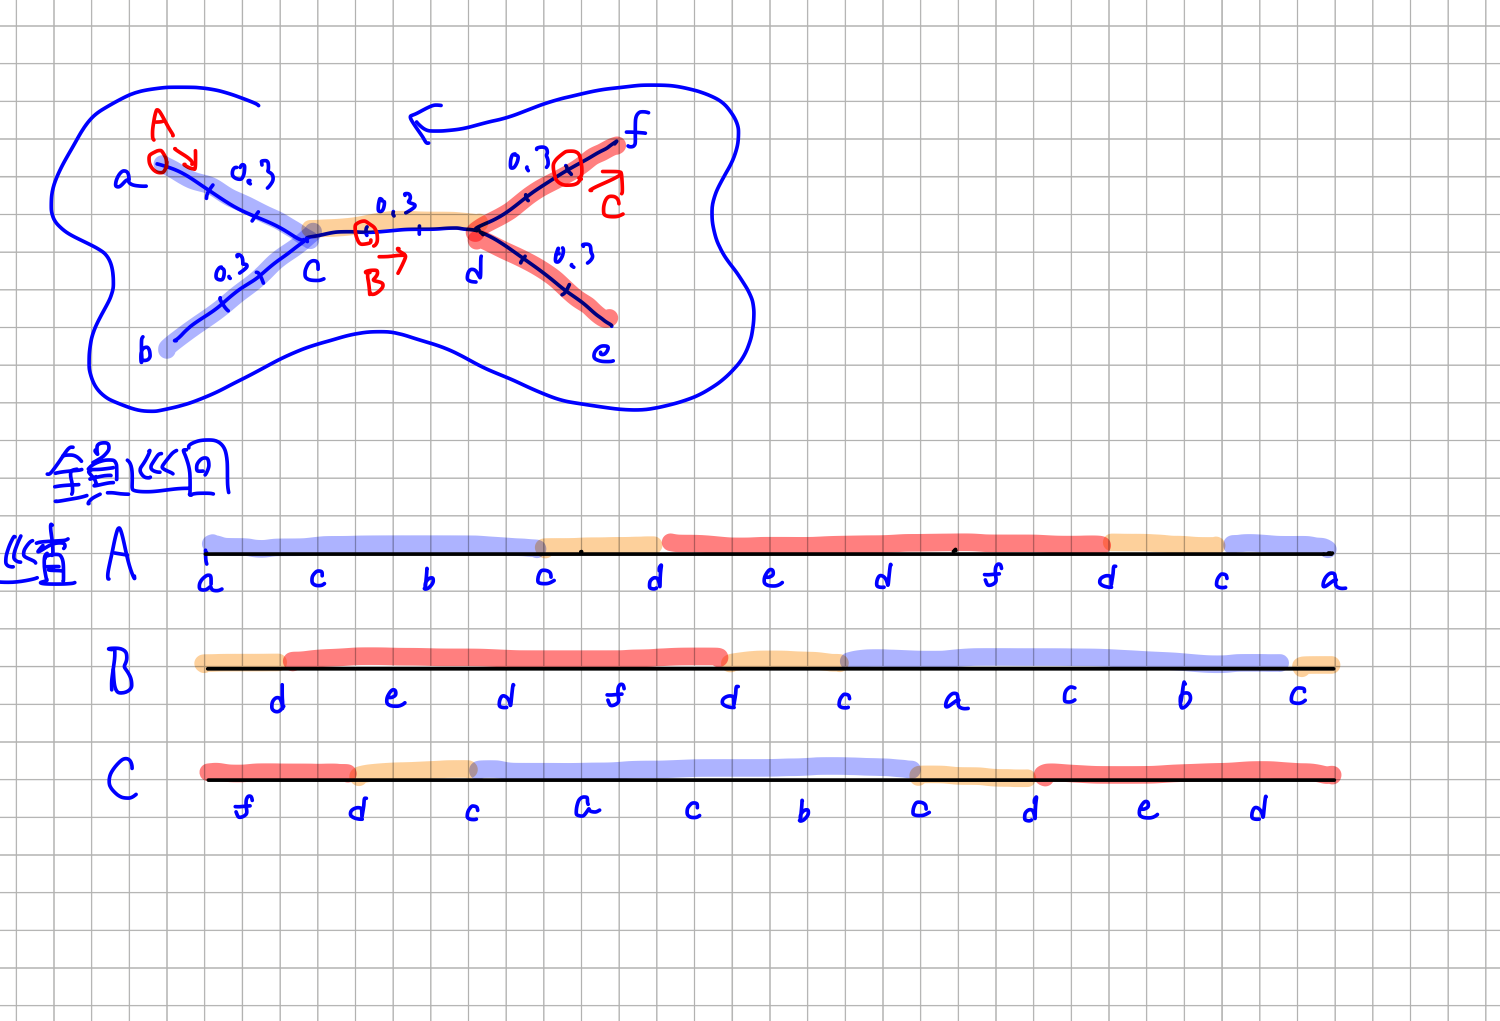
\includegraphics[scale=0.3]{\figdir/tree_memo_001.jpeg}
\end{figure}

\subsubsection{2017/10/10}
\begin{itemize}
  \item 星2つの中心同士が1本の橋で結ばれた図形をまず考える.
  \item 【予想】左右独立運行 or 全員協力運行のいずれかが最適になる
  \item 簡単な場合から
  \begin{itemize}
    \item 長い枝は省く(1人常駐が必要なのは示せそう)
    \item 左右の星は同じ図形の場合
    \item さらに枝の長さをすべて同じにする
  \end{itemize}

  \item $m$人による全員協力運行で警邏可能であるとき,
    \[
      2(\sum_{e \in E} d(e) + b) \leq mQ
    \]
    where
      $Q$:{\idletime},
      $m$:巡査の人数,
      $b$:橋の長さ,
      $E$:枝の集合.
    (逆も成立)

  \item $m$人による左右独立運行で警邏可能であるとき,
    ある$k (0 < k < m)$が存在し,
    \[
      2 \sum_{e \in L} d(e) \leq kQ
      \text{かつ}
      2 \sum_{e \in R} d(e) \leq (m - k)Q
    \]
    where
      $Q$:{\idletime},
      $m$:巡査の人数,
      $b$:橋の長さ,
      $L$:左の星の枝の集合,
      $R$:右の星の枝の集合.
    (逆も成立)
\end{itemize}



\subsubsection{2017/10/17}
\begin{itemize}
  \item 運行の帰着で示すのが難しそう(仮説の運行は複数人の動きを同時に決めているので).
  \item 1度も橋を渡らない運行では左右独立運行が最適.
  \item 1度でも橋を渡る運行では全員協力運行より少ない人数では警邏できないことを示す?
  \item {\idletime}$Q$ごとに橋往復の$2b$のコストがかかることを示せればよい
\end{itemize}


\subsubsection{2017/10/18}
\begin{itemize}
  \item 左右それぞれの星は最小$m_L, m_R$人で警邏できるとすると,
    あえて橋を渡るのは$m_L + m_R - 1$人以下にできる場合のみ.
    すると,少なくとも一方は警邏可能最小人数より1人以上少ない巡査で
    運行する時間が生まれる.この時間の上限はいくらか.

\end{itemize}

